\cleardoubleoddpage
\chapter{Experimental Setup}
\label{chap:experimental-setup}

This chapter describes the experimental design for both evaluation tracks,
answering the research questions posed in
Chapter~\ref{chap:introduction}.
Sections~\ref{sec:exp:datasets}--\ref{sec:exp:protocol} cover the
CIFAR-10 track; Section~\ref{sec:exp:inkjet} covers the inkjet pipeline.

%% ------------------------------------------------------------------

\section{Datasets}
\label{sec:exp:datasets}

\subsection{In-Distribution Dataset: CIFAR-10}
\label{sec:exp:datasets:id}

\paragraph{Dataset description.}
CIFAR-10~\cite{krizhevsky2009learning} consists of 60,000
$32 \times 32$ colour images across 10 classes: airplane, automobile,
bird, cat, deer, dog, frog, horse, ship, and truck.

\paragraph{Binary split.}
We adopt a binary framing: the airplane class (class~0) forms the
in-distribution set, and the remaining nine classes form the OOD proxy.
This yields a controlled binary OOD problem where the ID/OOD boundary is
known.

\paragraph{Data splits.}
\begin{itemize}
  \item Training set: 45,000 images (90\% of original 50,000 training
        images, stratified)
  \item Validation set: 5,000 images (10\% of training, stratified)
  \item Test set: 10,000 images (standard CIFAR-10 test set)
\end{itemize}

\paragraph{Preprocessing.}
All images are converted to PyTorch tensors, normalised to $[-1, 1]$ via
$x' = 2x - 1$, and augmented during training with random horizontal
flips. Validation and test sets receive only normalisation.

We evaluate on seven candidate OOD datasets spanning near- to far-OOD
distributional distances from CIFAR-10.

\textbf{Near-OOD: CIFAR-100}~\cite{krizhevsky2009learning} (10,000 test images,
$32 \times 32$, 100 classes sharing CIFAR-10 image statistics);
STL-10~\cite{coates2011analysis} (8,000 images, resized to
$32 \times 32$, overlapping classes with CIFAR-10).

\textbf{Far-OOD: Food-101}~\cite{bossard2014food} (25,250 images, resized to
$32 \times 32$); SVHN~\cite{netzer2011reading} (26,032 digit images,
$32 \times 32$); \textbf{FashionMNIST}~\cite{xiao2017fashion} (10,000 greyscale
clothing images, resized to $32 \times 32$, converted to 3-channel);
\textbf{Textures (DTD)}~\cite{cimpoi2014describing} (1,880 texture images,
cropped and resized to $32 \times 32$);
\textbf{Places365}~\cite{zhou2018places} (10,000 scene images,
$32 \times 32$). All datasets are normalised to $[-1, 1]$.

Under the final audit policy, core external claims use the five datasets
with recoverable current raw-score tensors (CIFAR-100, Places365,
FashionMNIST, SVHN, Textures); Food-101 and STL-10 are retained as
legacy traceability entries only.

\subsection{Dataset Statistics}
\label{sec:exp:datasets:statistics}

\begin{table}[htbp]
  \centering
  \caption{Dataset statistics for in-distribution and
    out-of-distribution datasets, spanning near-OOD (shared visual
    statistics) to far-OOD (distinct domains) evaluation scenarios.}
  \label{tab:exp:dataset-statistics}
  \begin{tabular}{llrrl}
    \toprule
    Dataset & Type & Test Images & Classes & Resolution \\
    \midrule
    CIFAR-10 (airplane) & ID          &  1,000 &   1 & $32 \times 32$  \\
    CIFAR-10 (rest)     & OOD proxy   &  9,000 &   9 & $32 \times 32$  \\
    CIFAR-100           & Near OOD    & 10,000 & 100 & $32 \times 32$  \\
    Places365           & Far OOD     & 10,000 & 365 & $32 \times 32$  \\
    STL-10              & Near OOD    &  8,000 &  10 & $96 \times 96$  \\
    Food-101            & Far OOD     & 25,250 & 101 & Variable        \\
    SVHN                & Far OOD     & 26,032 &  10 & $32 \times 32$  \\
    FashionMNIST        & Far OOD     & 10,000 &  10 & $28 \times 28$  \\
    Textures (DTD)      & Far OOD     &  1,880 &  47 & Variable        \\
    \bottomrule
  \end{tabular}
\end{table}

%% ------------------------------------------------------------------

\section{Experimental Design}
\label{sec:exp:design}

\subsection{Primary Experiment: Binary CDM Robustness Across Seeds}
\label{sec:exp:design:primary}

We train the binary conditional diffusion model with three random seeds
($\{42, 123, 456\}$) using the separation loss weight
$\lambda = 0.01$ and $K = 50$ Monte Carlo trials at inference. The three
seeds control model initialisation, data shuffling, and all stochastic
training operations.

\paragraph{Research question:}
Is the binary CDM's OOD detection performance stable across training
runs, and what is its mean AUROC and standard deviation on the
within-CIFAR binary test split?

\paragraph{Evaluation:}
Within-CIFAR AUROC and FPR@95\%TPR are the primary metrics. For the
final audited report, core claims are restricted to results with
recoverable raw-score artefacts (seed-42 raw-score evaluation for
external OOD; $K = 100$ MC trials).

\subsection{Separation Loss Ablation}
\label{sec:exp:design:separation}

We conduct a complete sweep over six separation loss weights:
$\lambda \in \{0.0, 0.001, 0.01, 0.02, 0.05, 0.1\}$. The reference
weight $\lambda = 0.01$ is evaluated with three seeds
(seeds 42/123/456); $\lambda = 0.02$ is also evaluated with three seeds.
All other $\lambda$ values are evaluated with seed~42 only. Each
$\lambda$ value is additionally evaluated on SVHN to assess
cross-domain stability.

\paragraph{Research question:}
How much does the separation loss improve OOD detection, and what is the
optimal weight $\lambda$?

\subsection{Ablation 1: Number of Monte Carlo Trials ($K$)}
\label{sec:exp:design:mc-trials}

We vary the number of timestep samples
$K \in \{1, 5, 10, 25, 50, 100\}$ used to compute the OOD score
(seed-42 checkpoint, $\lambda = 0.01$).

\paragraph{Research question:}
What is the accuracy--efficiency trade-off as $K$ increases, and what is
the minimum $K$ for near-optimal performance?

\paragraph{Evaluation:}
AUROC, FPR@95\%TPR, and wall-clock inference time (seconds per 10K
images on a single NVIDIA V100 GPU).

\subsection{Ablation 2: Timestep Sampling Strategy}
\label{sec:exp:design:timestep}

We compare three strategies for sampling timesteps during OOD scoring
(seed-42 checkpoint, $\lambda = 0.01$, $K = 50$):
\begin{itemize}
  \item \textbf{Uniform:} $t \sim \mathcal{U}[1, T]$ uniformly
  \item \textbf{Mid-focus:} Truncated normal
        $t \sim \mathcal{N}_{\mathrm{trunc}}(\mu = 300, \sigma = 150)$
  \item \textbf{Stratified:} Divide $[1, T]$ into $K$ equal bins; sample one $t$
        per bin
\end{itemize}

\paragraph{Research question:}
Which noise-level coverage is most informative for OOD detection?

\subsection{Ablation 3: OOD Scoring Method}
\label{sec:exp:design:scoring}

We compare three scoring formulations (seed-42 checkpoint,
$\lambda = 0.01$, $K = 50$):
\begin{itemize}
  \item \textbf{Difference:} $s(x) = e_0(x) - e_1(x)$ (ID error minus OOD error)
  \item Ratio: $s(x) = e_0(x) / e_1(x)$ (ID error divided by OOD error)
  \item \textbf{ID error only:} $s(x) = e_0(x)$ (no contrastive comparison)
\end{itemize}

\paragraph{Research question:}
Is contrastive scoring (using both binary conditions) essential, and do
difference and ratio scoring differ significantly?

%% ------------------------------------------------------------------

\section{Implementation Details}
\label{sec:exp:implementation-details}

\subsection{Binary CDM Architecture}
\label{sec:exp:impl:binary-cdm}

The binary CDM uses a UNet backbone with base channel width~128, channel
multipliers $[1, 2, 2, 4]$ (yielding channels $[128, 256, 256, 512]$),
attention at resolutions $16 \times 16$ and $8 \times 8$, two residual
blocks per resolution, and class-conditional Adaptive Group
Normalisation (AdaGN); full architectural details are provided in
Chapter~\ref{chap:implementation}
and Appendix~\ref{app:experimental-config}.
The model has ${\sim}68.8$\,M trainable parameters with binary
conditioning ($c = 0$: airplane, $c = 1$: rest).

\paragraph{Noise schedule.}
Cosine schedule~\cite{nichol2021improved} with $T = 1000$ timesteps:
$\bar{\alpha}_t
  = \cos^2\!\left(\frac{t/T + s}{1 + s} \cdot \frac{\pi}{2}\right)$,
$s = 0.008$.

\paragraph{Training configuration.}
\begin{itemize}
  \item Optimiser: AdamW ($\beta_1 = 0.9$, $\beta_2 = 0.999$,
        $\varepsilon = 10^{-8}$, weight decay
        $\lambda_{\mathrm{wd}} = 0.01$)
  \item Learning rate: $10^{-4}$ with 5-epoch linear warm-up then cosine
        annealing
  \item Batch size: 128
  \item Classifier-free guidance dropout:
        $p_{\mathrm{uncond}} = 0.1$
  \item Early stopping: patience 30 epochs on validation AUROC
  \item Hardware: Single GPU per run (V100 16\,GB, GV100 32\,GB, or
        P40 24\,GB); training time $\approx$ 10--16\,h on GV100,
        ${\sim}$18--28\,h on V100/P40
\end{itemize}

\paragraph{OOD scoring.}
Default: $K = 50$ MC trials, uniform timestep sampling, difference
scoring. External OOD evaluation uses $K = 100$ for higher stability.

\paragraph{Separation loss.}
During training, the separation loss $\mathcal{L}_{\text{sep}}$
(Equation~\ref{eq:meth:lsep}) is added with weight $\lambda$ as part of
the total training objective
(Equation~\ref{eq:meth:ltotal}). The separation loss is computed on each
mini-batch using the predicted noise errors under both conditions.

\subsection{Inkjet CDM Architecture}
\label{sec:exp:impl:inkjet-cdm}

The inkjet CDM uses the same diffusion-scoring principle as the CIFAR
model but a separate custom \texttt{NoisePredictorV3} UNet tailored to
$128 \times 128$ feature crops. It uses a multi-head conditioning
mechanism:
\begin{itemize}
  \item Template type embedding (3 values: A, B, C)
  \item Feature type embedding (8 values: dist1, dist6, edge1--edge4,
        angle, dots)
  \item Quality label embedding (2 values: GOOD, BAD)
  \item Bounding box coordinates (4 values, normalised)
\end{itemize}

Input resolution: $128 \times 128$ (YOLO-cropped feature patches).
Training uses stratified 5-fold CV with image-level splitting. The
public implementation defaults to $K=50$ inference trials, while the
retained separation-loss ablation reported in Chapter~\ref{chap:results}
uses $K=100$ to reduce Monte Carlo scoring variance.

%% ------------------------------------------------------------------

\section{Evaluation Protocol}
\label{sec:exp:protocol}

\subsection{Metrics}
\label{sec:exp:protocol:metrics}

\textbf{Primary metrics:} AUROC (overall discrimination; $1.0$ = perfect,
$0.5$ = random) and FPR@95\%TPR (false positive rate at 95\% true positive
rate; lower is better). Formal definitions, including the TPR/FPR
equations, are provided in Section~\ref{sec:meth:problem:metrics};
AUPRC and Detection Error are reported for completeness.

\textbf{Reporting:} Seed-level CIFAR analyses with $n < 5$ are reported
descriptively (no inferential significance claims). For inkjet
($n = 5$ folds), significance uses paired $t$-test and Wilcoxon
signed-rank tests with Holm correction.

\subsection{Within-CIFAR Evaluation}
\label{sec:exp:protocol:within-cifar}

For the within-CIFAR binary test split: ID samples are the 1,000
CIFAR-10 test images of the airplane class. OOD samples are the 9,000
CIFAR-10 test images of the nine remaining classes. AUROC is computed
using scikit-learn with default parameters.

\subsection{External OOD Evaluation}
\label{sec:exp:protocol:external-ood}

For each external OOD dataset: the reference pool is the full CIFAR-10
test set (10,000 images), because the binary CDM was trained on both
conditional branches of CIFAR-10: airplane as $c{=}0$ and the
remaining nine classes as $c{=}1$. OOD samples are the full external
dataset test split. Scores are computed with $K = 100$ MC trials. AUROC and
FPR@95\%TPR are reported for auditable raw-score runs. Datasets without
recoverable current raw-score tensors are retained only as legacy
traceability entries and excluded from core claims. Importantly, no
external OOD data was used for threshold calibration, hyperparameter
selection, or early stopping; all model selection was performed on the
within-CIFAR validation split (Section~\ref{sec:bg:ood}).

\subsection{Reproducibility}
\label{sec:exp:protocol:reproducibility}

All experiments use deterministic PyTorch settings:

\medskip
\noindent
\texttt{torch.backends.cudnn.deterministic = True}\\
\texttt{torch.use\_deterministic\_algorithms(True)}

\medskip
Each checkpoint saves model state, EMA state, optimiser state, and
training step. The best validation AUROC checkpoint is used for all
evaluations. Training and evaluation scripts for the CIFAR-10 experiments are
available at \url{https://github.com/ahmed-3m/DiffusionOOD}; pre-trained
model weights (all seeds and $\lambda$ configurations) are hosted at
\url{https://huggingface.co/ahmed-3m/DiffusionOOD}, enabling direct
evaluation without retraining. The inkjet CDM scripts are reproducible
from the public \texttt{InkjetOOD}
repository~\cite{mohammed2026inkjetood} at commit \texttt{c34daf8};
the corresponding pre-trained inkjet CDM weights are available at
\url{https://huggingface.co/ahmed-3m/InkjetOOD}. Both tracks also
require the public PROFACTOR FTI\_Zer0P dataset on
Zenodo~\cite{profactor2024fti}. After downloading the dataset, the
expected layout is \texttt{data/images/} for PNG files and
\texttt{data/metadata.csv} with columns \texttt{file\_name},
\texttt{label}, and \texttt{feature}. The repository documents
training, evaluation, 5-fold cross-validation, and figure-regeneration
commands for the retained inkjet CDM results.
The corresponding public command sequence is:

\begin{verbatim}
git clone https://github.com/ahmed-3m/InkjetOOD.git
cd InkjetOOD
git checkout c34daf8b00a3e77252f2b70b79ac0ec99342da5b
pip install -r requirements.txt
python run_ablation.py --metadata ./data/metadata.csv --img_dir ./data/images
python run_cv.py --metadata ./data/metadata.csv --img_dir ./data/images
python scripts/plot_inkjet_results.py
\end{verbatim}

Single-run reproduction can also be performed with
\texttt{python train.py --metadata ./data/metadata.csv --img\_dir
./data/images --sep\_loss\_weight 0.01 --eval\_after} followed by
\texttt{python evaluate.py --checkpoint results/train/cdm\_best.pt
--metadata ./data/metadata.csv --img\_dir ./data/images --num\_trials
100}.

%% ------------------------------------------------------------------

\section{Inkjet Print Quality Control Experiments}
\label{sec:exp:inkjet}

\subsection{Dataset}
\label{sec:exp:inkjet:dataset}

The public FTI\_Zer0P inkjet print quality
dataset~\cite{profactor2024fti} contains 1,204 inkjet print images
captured from 15 building components, organised into 53 print datasets
with up to three print areas per component. Of these images, 960 are
labelled as GOOD or BAD for the relevant print-quality features.

\paragraph{Feature extraction.}
YOLOv8n detects and crops features from template images; each crop is
labelled with template type, feature type, quality label (GOOD/BAD), and
bounding box coordinates.

\begin{figure}[htbp]
  \centering
  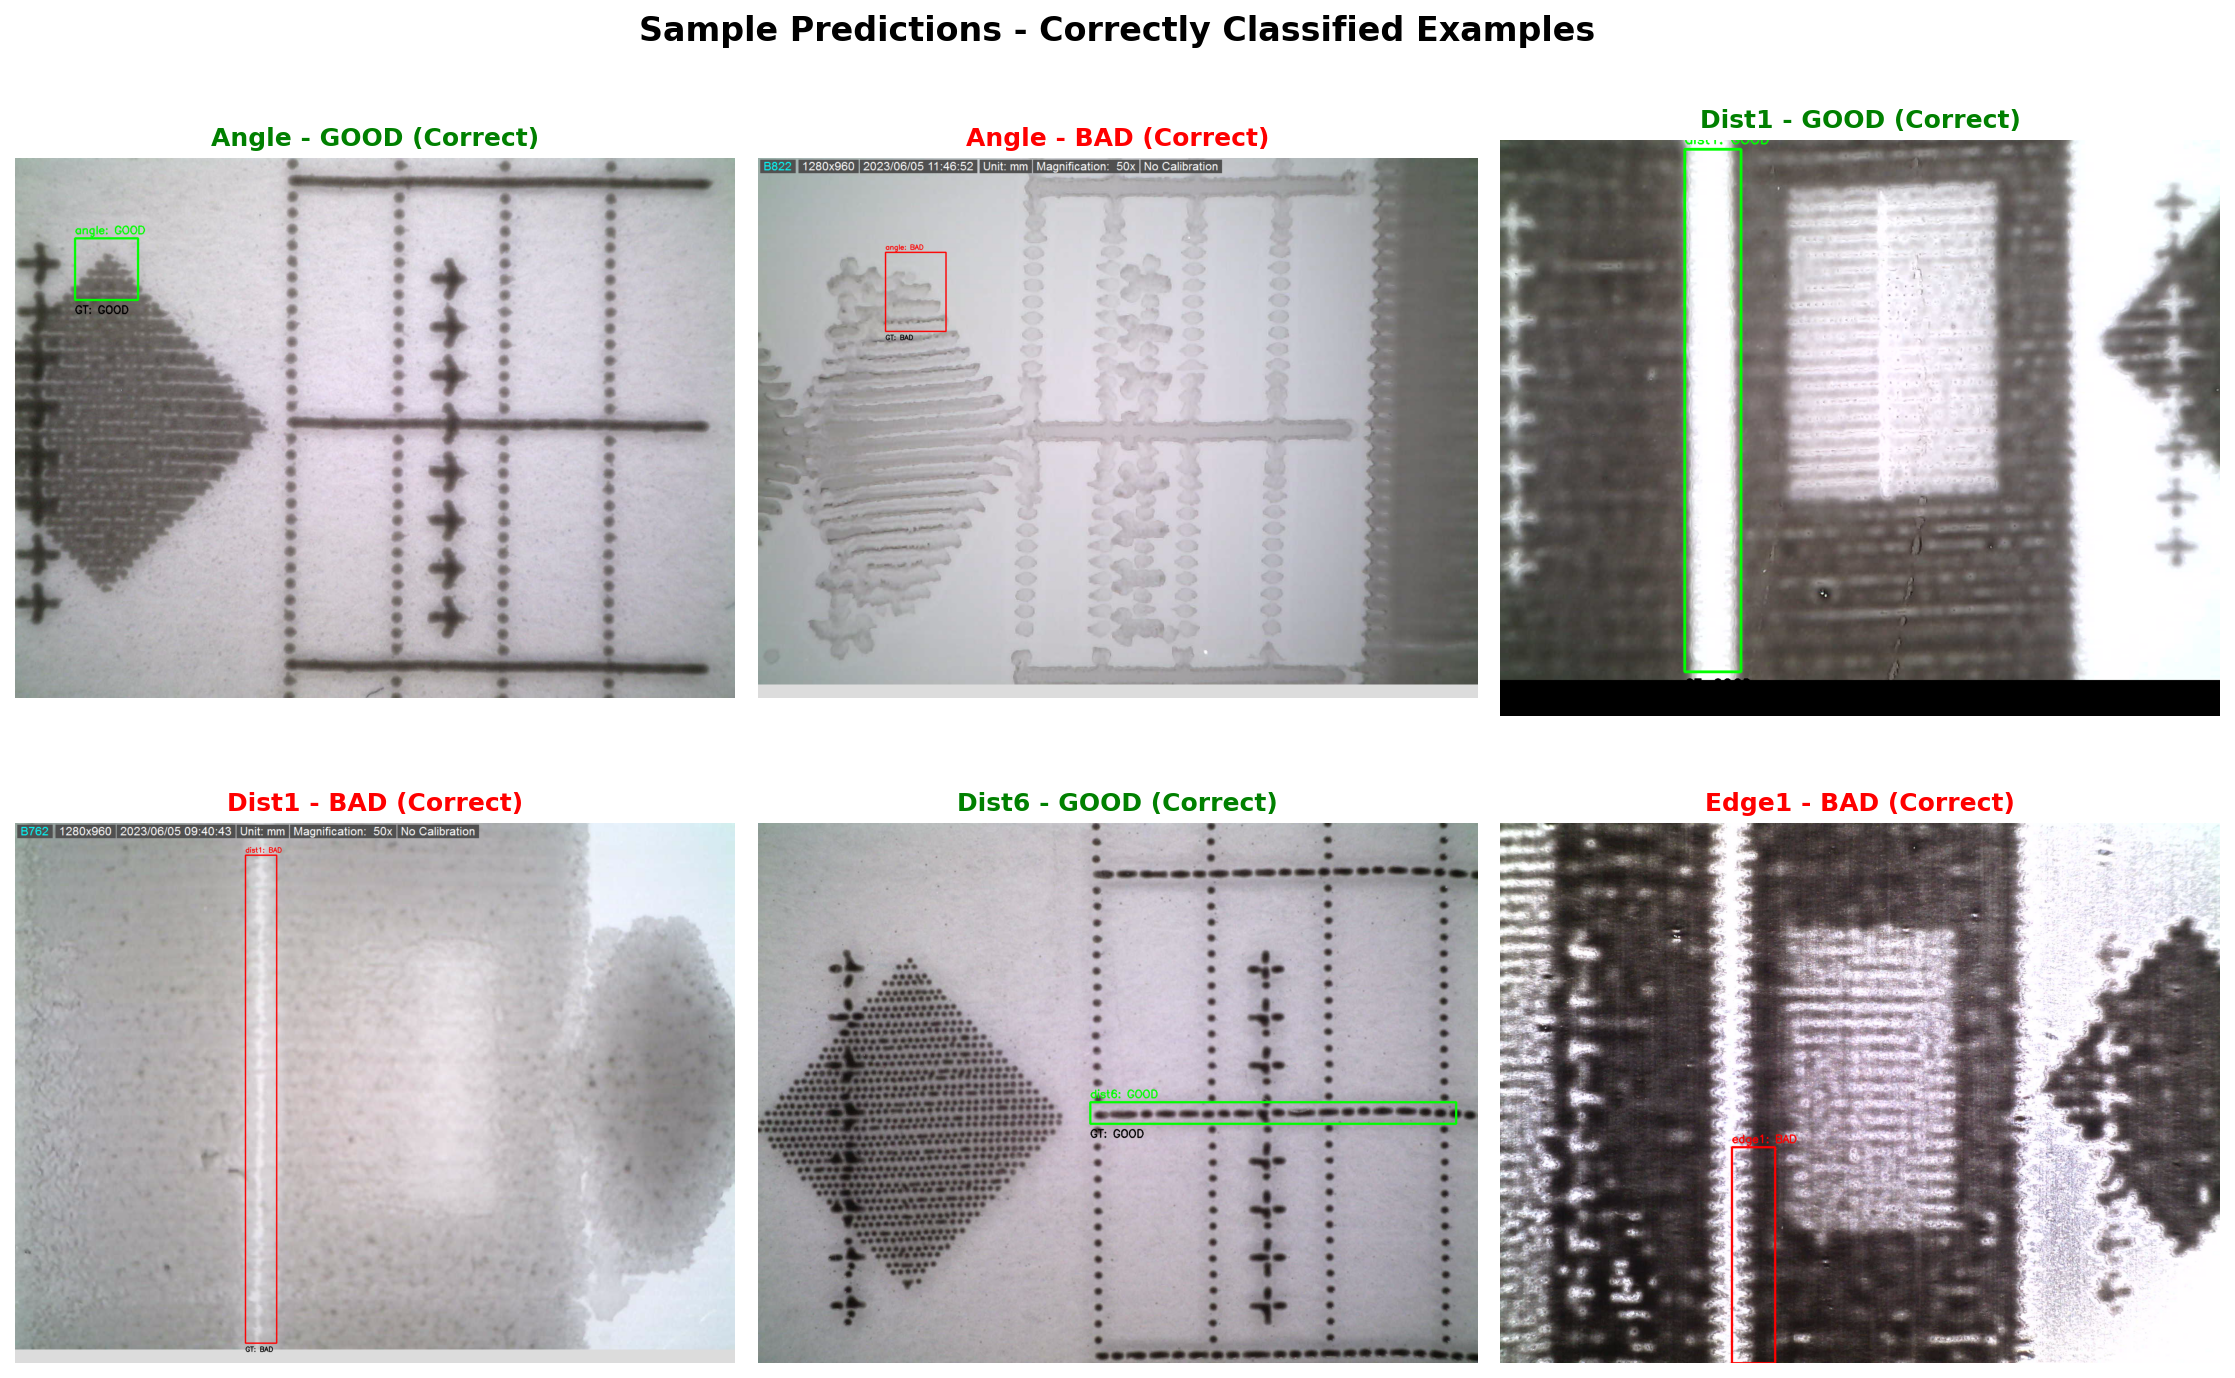
\includegraphics[width=\textwidth]{images/fig_inkjet_examples.png}
  \caption{Example images from the inkjet print quality dataset with
    YOLO detections and CDM predictions. Green bounding boxes indicate
    GOOD quality predictions; red boxes indicate BAD quality predictions.
    Feature types shown: angle, dist1, dist6, edge.}
  \label{fig:exp:inkjet-examples}
\end{figure}

\begin{table}[htbp]
  \centering
  \caption{Inkjet print quality dataset statistics. Public dataset
    counts follow the Zenodo record; retained CDM evaluation counts
    describe the processed YOLO feature-crop representation.}
  \label{tab:exp:inkjet-statistics}
  \begin{tabular}{ll}
    \toprule
    Property & Value \\
    \midrule
    Public images       & 1,204 \\
    Public labelled images & 960 \\
    Building components & 15 \\
    Print datasets      & 53 \\
    Processed source-image groups & 573 \\
    Resolution          & $1920 \times 1080$ pixels \\
    Template types      & 3 (A, B, C) \\
    Feature types       & 8 (dist1, dist6, edge1--edge4, angle, dots) \\
    Quality labels      & 2 (GOOD, BAD) \\
    Retained feature-level crops & 6,408 \\
    GOOD\,:\,BAD ratio  & ${\sim}2{:}1$ overall (varies by feature) \\
    \bottomrule
  \end{tabular}
\end{table}

\noindent\textbf{Per-Feature Class Balance (GOOD\,:\,BAD ratio):}
\begin{itemize}
  \item dist1: 1.82\,:\,1
  \item dist6: 1.94\,:\,1
  \item edge1--edge4: 1.68\,:\,1--2.31\,:\,1
  \item angle: 9.67\,:\,1 (most imbalanced)
  \item dots: 3.45\,:\,1
\end{itemize}

\subsection{Methods Under Comparison}
\label{sec:exp:inkjet:methods}

The retained public experiment is the \textbf{YOLO\,+\,CDM} pipeline:
YOLOv8n detects feature regions, and a multi-head CDM classifies each
crop via differential reconstruction error under GOOD and BAD quality
conditions. Earlier internal supervised and anomaly-detection baselines
are excluded from the retained thesis evidence because their complete
public code, splits, configurations, and results are not released in the
submission artefacts. The public experiment therefore reports only
results that can be regenerated from \texttt{InkjetOOD}, the public
FTI\_Zer0P dataset, and the released CDM weights.

\subsection{Evaluation Protocol}
\label{sec:exp:inkjet:evaluation}

\paragraph{Cross-validation.}
Stratified 5-fold cross-validation with image-level splitting across the
573 processed source-image groups; all feature crops from the same
source image remain in the same fold, preventing data leakage. Separation
loss ablation: the CDM is
trained with $\lambda \in \{0.0, 0.01, 0.02, 0.05\}$ to evaluate
whether the separation loss improves inkjet quality classification.

\paragraph{Metrics.}
Primary: AUROC (mean $\pm$ std across 5 folds); secondary: Accuracy, F1,
Precision, Recall. Paired $t$-tests and Wilcoxon signed-rank tests are
reported for $\lambda$ differences, with Holm correction for multiple
comparisons. All retained public CDM evaluations use the same image-level
splits, the same YOLO detections, and the same evaluation codepath.
